\documentclass[a4paper]{article}

%% Language and font encodings
\usepackage[utf8]{inputenc}
\usepackage[T1]{fontenc}
\usepackage{polski}
\usepackage{amssymb}


%% Sets page size and margins
\usepackage[a4paper,top=3cm,bottom=3cm,left=3.5cm,right=3.5cm,marginparwidth=2cm]{geometry}

%% Useful packages
\usepackage{amsmath}
\usepackage{graphicx}
\usepackage[colorinlistoftodos]{todonotes}
\usepackage[colorlinks=true, allcolors=blue]{hyperref}
\usepackage{listings}

\graphicspath{{./fig/}}

\title{ALHE - Raport z projektu}
\author{Kaczmarek Kamil, Lewczuk Grzegorz}

\begin{document}
\maketitle

\begin{abstract}
Analiza problemu utworzenia sieci autostrad pomiędzy miastami oraz implementacja algorytmu optymalizującego rozwiązanie.
\end{abstract}

\section{Opis zagadnienia}

\begin{quote}
Przygotować algorytm poszukujący optymalnej sieci autostrad tworzącą siatkę połączeń pomiędzy miastami z danego zbioru - położenia miast są nam znane. Rozwiązanie powinno uwzględniać miejsca zjazdów (nie mogą one znajdować się zbyt blisko siebie) oraz pozwalać na przecinanie się autostrad nie tylko w miastach.
\end{quote}

\section{Zmiany dotyczące założeń}

Wprowadzono następujące zmiany w założeniach projektu w celu poprawności działania implementacji problemu:

\begin{itemize}
\item Przestrzeń została ograniczona do kwadratu o wymiarach 101x101 – współrzędne x,y z zakresu [0, 100].
\item Współrzędne miast i wierzchołki łamanej budującej autostradę są liczbami całkowitymi, natomiast wyliczane punkty zjazdu mogą być punktami o współrzędnych rzeczywistych.
\item Losowy sąsiad dla punktów z przestrzeni poszukiwań jest wyznaczany poprzez wylosowanie jednego z wierzchołków autostrady. Następnie losowane są dla niego nowe współrzędne x, y oraz parametr w, który oznacza numer wierzchołka autostrady, z którym jest połączony dany punkt.
\item Funkcja kosztu jest obliczana zgodnie założeniami dokumentacji wstępnej. Doprecyzowaniu uległa jedynie kara za niezachowanie spójności autostrady, która została ustalona jako 1e100.
\end{itemize}

\section{Implementacja}

Do implementacji projektu użyto języka Python 3.6 wraz z dodatkowymi bibliotekami:
\begin{itemize}
\item matplotlib - wyświetlanie wyników w formia graficznej na wykresie.
\item numpy - wykonywanie obliczeń i przekształceń na wektorach.
\item argparse - przygotowanie argumentów wprowadzanych podczas uruchomienia programu.
\item simanneal - zewnętrzna implementacja algorytmu symulowanego wyżarzania, opisanego poniżej.
\end{itemize}

\subsection{Model}

Utworzono klasę modelu, zawierającą atrybuty:
\begin{itemize}
\item listę miast, z której łatwo także wyznaczć liczbę miast M,
\item listę punktów autostrady, z której łatwo wyznaczyć liczbę punktów autostrady K,
\item wartość minimalnej odległości pomiędzy zjazdami,
\item pomocniczą listę punktów zjazdów z autostrady.
\end{itemize}

Dodatkowo w modelu zdefiniowane są metody pozwalające na znalezienie sąsiada oraz obliczenia funkcji kosztu używane w algorytmie symulowanego wyżarzania. Oprócz tego są także metody pomocnicze.

\subsection{Uruchamianie}

Dzięki modułowi argparse, zdefiniowano interfejs użytkownika pozwalający na dodanie w prosty sposób argumentów wywołania programu. Plik główny projektu, to \texttt{main.py}. Dodano do niego linijkę \texttt{\#!/usr/bin/env python}, aby był możliwy do uruchomienia z poziomu powłoki.

Po wpisaniu \texttt{./main.py -h} mozna uzyskać pomoc dotyczącą działania programu:
\begin{lstlisting}[basicstyle=\ttfamily\selectfont\footnotesize]
usage: main.py [-h] [-s STEPS] [--show] cities k d

Highway system

positional arguments:
  cities                filename with cities positions, "random" for random
                        cities
  k                     number of highway points
  d                     minimal distance between exits

optional arguments:
  -h, --help            show this help message and exit
  -s STEPS, --steps STEPS
                        steps to perform
  --show                show model through iterations
\end{lstlisting}

Obowiązkowe jest podanie nazwy pliku zawierającego współrzędne miast, liczby k punktów autostrad oraz wartości d minimalnej odległości pomiędzy zjazdami.\newline
Dodatkowo można podać liczbę kroków algorytmu STEPS oraz ustawić flagę \texttt{--show}, dzięki której można śledzić wyniki na bieżąco na wykresie.\newline
Istnieje także możliwość wywołania programu dla losowych miast, poprzez podanie w miejscu nazwy pliku z miastami słowa `random'. 

\subsection{Plik konfiguracyjny}

Program zawiera także plik konfiguracyjny określający wartości:
\begin{itemize}
\item domylna ilość miast - w przypadku tworzenia losowych współrzędnych.
\item maksymalne wartości współrzędnych X oraz Y.
\item ustawienia dotyczące algorytmu symulowanego wyżarzania.
\item wzór funkcji liniowej oraz wykładniczej kosztu.
\end{itemize}

\subsection{Wizualizacja wyników}

Do wizualizacji wyników użyto biblioteki matplotlib. Przykładowy wykres wygląda następująco.
\begin{figure}[h]
\centering
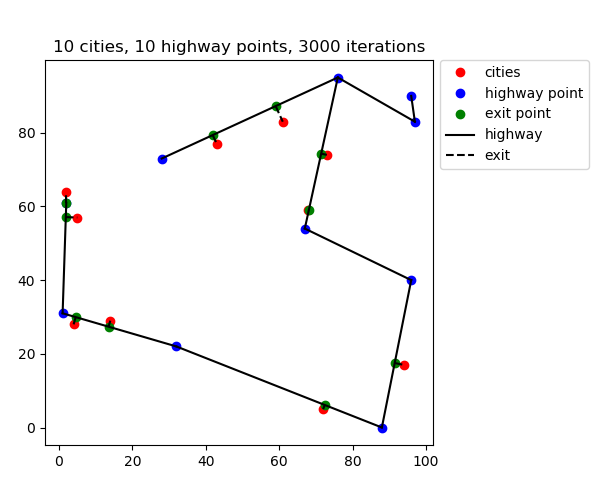
\includegraphics[width=12cm]{sample}
\caption{Wizualizacja wyników}
\end{figure}
Wszystkie oznaczenia oraz ustawienia opisane są na wykresie.



Dzięki temu możliwe jest w prosty sposób zmiana działania całego programu bez ingerencji w kod.


\section{Metaheurystyka}
Do minimalizacji funkcji kosztu autostrady zastosowano metodę optymalizacji symulowanego wyżarzania. Skorzystano z implementacji dostępnej w module simanneal dostępnej pod adresem \url{https://github.com/perrygeo/simanneal}. W celu zastosowania tego modułu należało zaimplementować metody move(), której zadaniem jest wybór punktu z sąsiedztwa punktu roboczego oraz metody energy(), która służy do obliczania funkcji celu dla danego punktu. Oprócz tego należało zdefiniować model, który zawierałby wszystkie dane wymagane do wykonywania funkcji move() oraz energy() zgodnie z założeniami projektu.
Metoda optymalizacji zawarta w module simanneal jest konfigurowana przez następujące parametry:
\begin{itemize}
\item Tmax – temperatura początkowa
\item Tmin – temperatura końcowa
\item Steps – liczba kroków algorytmu
\item Updates – parametr pomocniczy, który określa jak często wypisywać statystyki z dotychczasowego przebiegu algorytmu. Nie ma on wpływu na działanie metody optymalizacji.
\end{itemize}

Implementacja ta jest klasyczną wersją symulowanego wyżarzania. Przebieg kroku algorytmu jest następujący:
\begin{enumerate}
\item Wybierz punkt $y$ z sąsiedztwa punktu $x$ : $y$ = selRandom$(N(x))$
\item Jeśli $q(y) < q(x)$, to zapamiętaj punkt $y$ : $x = y$, gdzie $q()$ – funkcja celu
\item Jeśli $q(y) \ge q(x)$ i rand() < $p$, to również zapamiętaj punkt $y$: $x$ = $y$, 

gdzie $p$ = $exp\left(\frac{- |q(y)-q(x)|}{T}\right)$.
\item Algorytm kończy się po wykonaniu zdefiniowanej liczby kroków.
\item Temperatura zmienia się w kolejnych krokach zgodnie z zależnością:

$T = T_{max} * exp\left(\frac{T_{factor} * i }{steps}\right)$, gdzie:
\begin{itemize}
\item  $i$ – numer aktualnego kroku algorytmu
\item $T_{factor}$ – współczynnik obliczany w momencie inicjalizacji algorytmu
\item $T_{factor} = -log\left(\frac{T_{max}}{T_{min}}\right)$
\end{itemize}
Tak zdefiniowana temperatura zmienia się w czasie kolejnych kroków algorytmu od wartości $T_{max}$ do $T_{min}$. Jest to funkcja malejąca.
\end{enumerate}

\section{Temperatura}

W celu dobranie najlepszych parametrów temperatury przeprowadzono próby, których rezultat pokazany jest na poniższym wykresie:(M = 25, STEPS = 1000, k = 10, d = 0)
\begin{figure}[h]
\centering
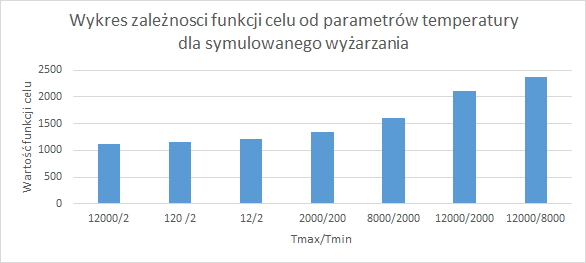
\includegraphics[width=12cm]{temp}
\caption{Wykres zależności funkcji celu od parametrów temperatury dla symulowanego wyżarzania}
\end{figure}\newline
Najlepsze wyniki otrzymano dla $T_{max}$=12000 oraz $T_{min}$=2.

\section{Testy}
Poprawność działania algorytmu została przetestowana na przykładzie o następujących założeniach. Przestrzeń zmniejszona do kwadratu o wymiarach 10x10, M=4, k=2, d=0.
\begin{figure}[h!]
\centering
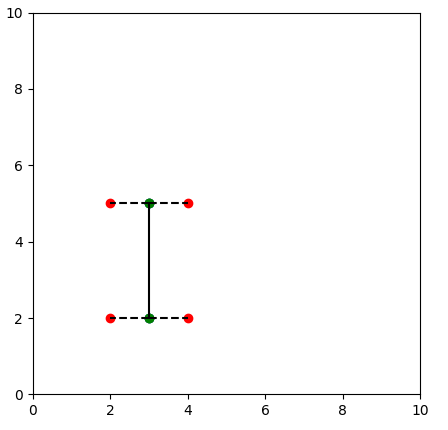
\includegraphics[width=6cm]{test}
\caption{Wynik podstawowego przypadku sprawdzającego poprawność algorytmu}
\end{figure}\newline
Dla liczby kroków steps = 10000 uzyskiwano rozwiązanie optymalne - minimum globalne funkcji kosztu wynoszące 7 (koszt autostrady = 3, koszt zjazdów = 4 * ($2^1$ - 1) = 4).\newline

Dodatkowo przetestowano przypadek dla M = 25 oraz K = 10 po wykonaniu 100 00 kroków algorytmu. Poniżej efekt.
\begin{figure}[h!]
\centering
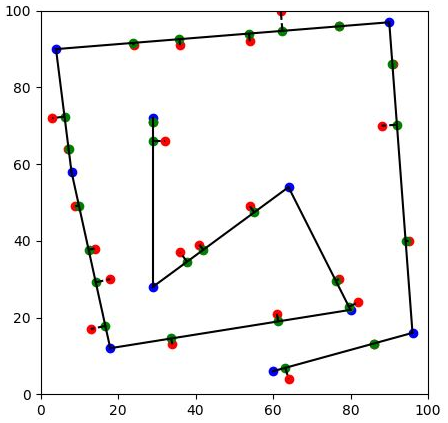
\includegraphics[width=6cm]{test2}
\caption{Przykładowy wynik działania algorytmu}
\end{figure}\newline
Po upewnieniu się, że model został poprawnie zdefiniowany dla metody optymalizacji przystąpiono do testów o większym rozmiarze problemu.

\subsection{Test 10 miast}

W pierwszym kroku sprawdzono przypadek dla 10 miast. Dodatkowe parametry to:
\begin{itemize}
\item M = 10
\item K = 10
\item D = 3
\item STEPS - zmienne od 10 do 10 000
\end{itemize}

Uzyskano następujące wartości funkcji celu w zależności od liczby kroków:
\begin{itemize}
\item 10 - 1801449.81
\item 100 - 7730.18
\item 1000 - 533.60
\item 10000 - 421.19
\end{itemize}

Można zauważyć bardzo szybki spadek wartości funkcji kosztu dla początkowych testów, później wartości wolniej się zmniejszają, ponieważ są już bliżej rozwiązania optymalnego.\newline
Poniżej grafika reprezentująca wyniki dla każdej z prób.
\begin{figure}[h!]
\centering
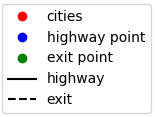
\includegraphics[width=3cm]{legend}
\caption{Legenda dla powstałych wizualizacji}
\end{figure}
\begin{figure}[h!]
\centering
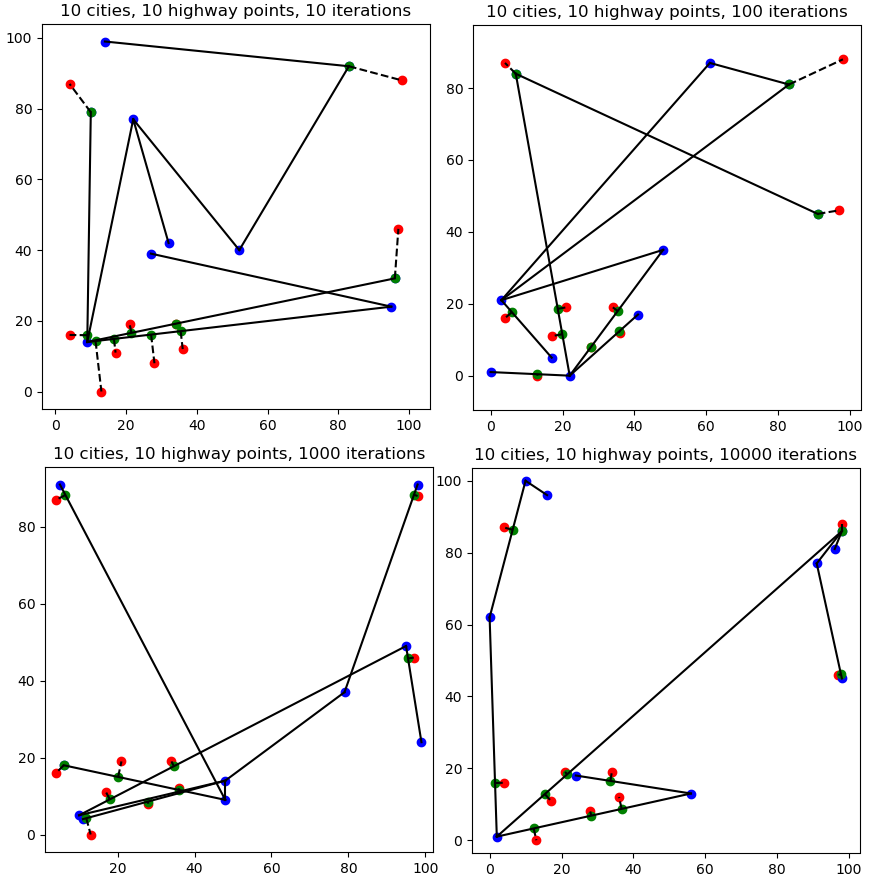
\includegraphics[width=12cm]{10_cities}
\caption{Wyniki dla 10 miast}
\end{figure}



\subsection{Test 25 miast}

W kolejnym kroku przeprowadzono testy kompleksowe zawierające więcej porównań. Dane początkowe:
\begin{itemize}
\item M = 25
\item K = 10
\item D = 0
\item STEPS - zmienne od 10 do 100 000
\end{itemize}
Dla każdej rozpatrywanej liczby kroków przeprowadzono po 10 niezależnych testów, a wynik minimalizacji kosztu autostrady widoczny na wykresie jest średnią z otrzymanych danych.
Dla liczby kroków STEPS = 100 000 czas działania algorytmu wynosił średnio 13 minut, natomiast dla steps = 10 000 około 1,5 min.\newline

Na podstawie wykresu przedstawionego na Rysunku~\ref{fig:wyk25} można zauważyć, że wartość funkcji celu sukcesywnie maleje wraz z ilością wykonanych kroków przez algorytm. Początkowe wartości są bardzo wysokie przez co nieakceptowalne. Jednak po wykonaniu ponad 1000 kroków wartości funkcji kosztu wolniej maleją, co oznacza że ciężej znaleźć lepsze rozwiązanie.
\vskip 5cm
\begin{figure}[h!]
\centering
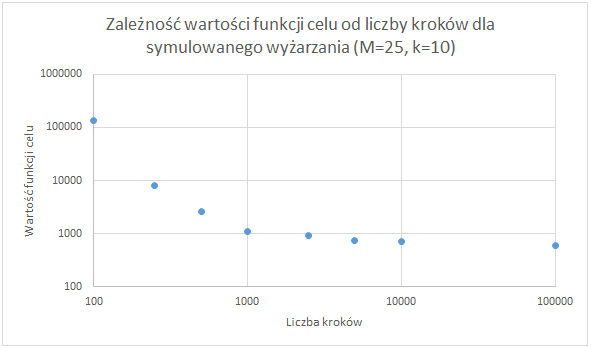
\includegraphics[width=12cm]{25_cities_wykres}
\caption{Wykres zależności funkcji celu od liczby kroków dla 25 miast}
\label{fig:wyk25}
\end{figure}
\vskip 1cm

Poniżej także wykresy prezentujące wyniki dla liczby kroków od 10 do 10000:

\begin{figure}[h!]
\centering
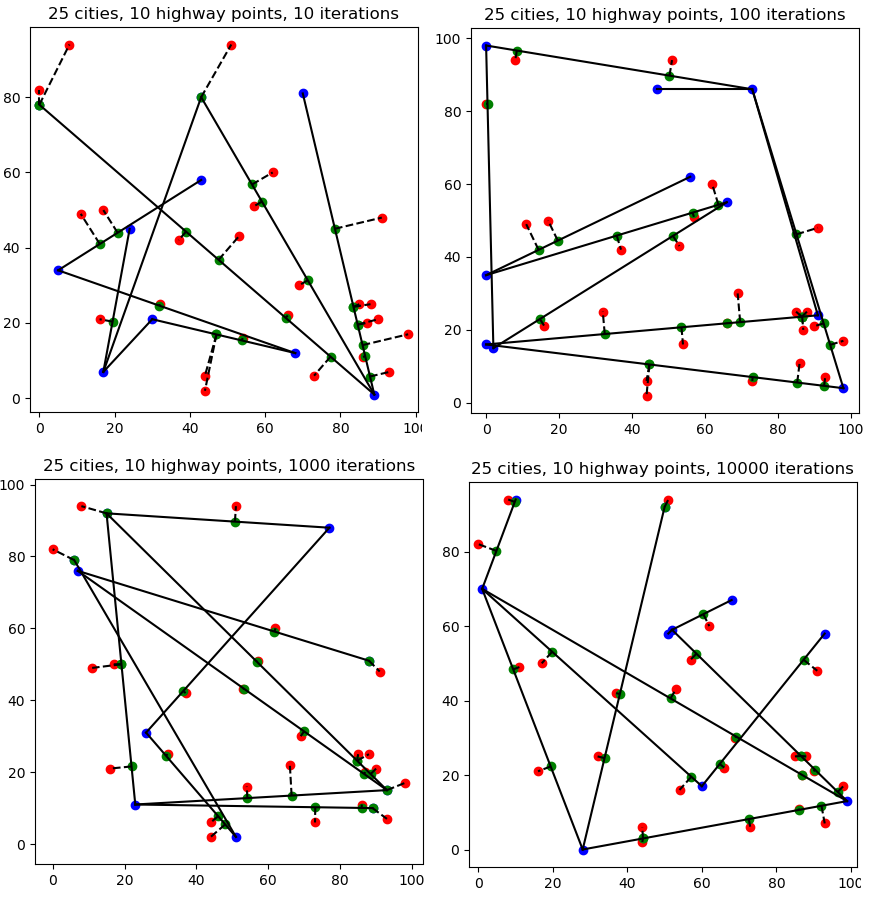
\includegraphics[width=12cm]{25_cities}
\caption{Wyniki dla 25 miast}
\end{figure}

Oraz uzyskane wartości funkcji celu w zależności od liczby kroków:
\begin{itemize}
\item 10 - 371075.61
\item 100 - 2027.27
\item 1000 - 1974.19
\item 10000 - 794.61
\end{itemize}

\subsection{Test 50 miast}

W ostanim przypadku przeprowadzono testy dla 50 miast. Dane początkowe:
\begin{itemize}
\item M = 50
\item K = 10
\item D = 0
\item STEPS - zmienne od 10 do 100 000
\end{itemize}

Podobnie jak w poprzednik przypadku, przeprowadzono wiele prób a wyniki uśredniono. Poniżej wykres zależności wartości funkcji celu od liczby kroków:
\begin{figure}[h!]
\centering
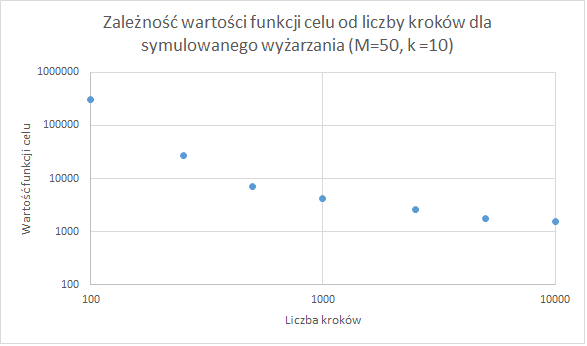
\includegraphics[width=12cm]{50_cities_wykres}
\caption{Wykres zależności funkcji celu od liczby kroków dla 50 miast}
\label{fig:wyk50}
\end{figure}

Poniżej wyniki funkcji celu dla przykładowego uruchomienia dla liczby kroków od 10 do 10 000:
\begin{itemize}
\item 10 - 4886132988.92
\item 100 - 130663.54
\item 1000 - 5062.10
\item 10000 - 1482.57
\end{itemize}

Oraz wizualizacja wyników:

\begin{figure}[h!]
\centering
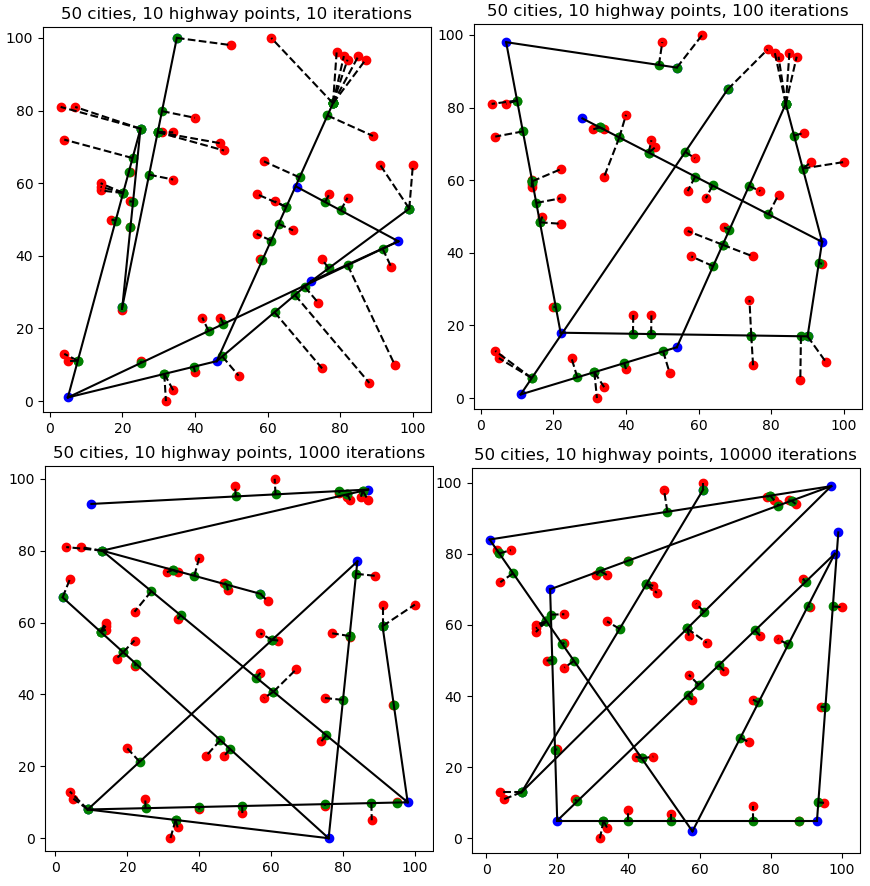
\includegraphics[width=12cm]{50_cities}
\caption{Wyniki dla 50 miast}
\end{figure}

\subsection{Uruchamianie testów}


Wszystkie testy mogą być w prosty sposób odtworzone na podstawie dostarczonych źródeł. W katalogu \texttt{tests} znajdują się podkatalogi zawierające współrzędne miast dla każdego testowanego przypadku. 

Dodatkowo utworzono skrytp \texttt{run\_tests.sh}, który wykona jeden przebieg wszystkich opisanych testów, dla ilości kroków 10, 100, 1000, 10 000. Dla każdego wyniku zostanie wyświetlony wynik w postaci wizualnej oraz utworzony plik zawierający uzyskane rozwiązanie, np. \texttt{tests/10\_cities/100steps}:
\begin{lstlisting}[basicstyle=\ttfamily\selectfont\footnotesize]
Cities: [(4, 87), (17, 11), (13, 0), (4, 16), (21, 19), (34, 19), 
(36, 12), (98, 88), (28, 8), (97, 46)]
Highway: [[(36, 53) -> (18, 31)], [(4, 25) -> (94, 48)], [(15, 12) -> (3, 74)],
 [(77, 29) -> (15, 12)], [(3, 74) -> (17, 30)], [(98, 91) -> (36, 53)], 
 [(94, 48) -> (98, 91)], [(17, 30) -> (36, 53)], [(13, 93) -> (98, 91)], 
 [(18, 31) -> (3, 74)]]
Total cost: 7730.180890387163
\end{lstlisting}

Cities, to współrzędne miast. Natomiast Highway to lista punktów na autostradzie w formacie [punkt -> następny punkt].



\end{document}